\documentclass[twoside]{book}

% Packages required by doxygen
\usepackage{fixltx2e}
\usepackage{calc}
\usepackage{doxygen}
\usepackage[export]{adjustbox} % also loads graphicx
\usepackage{graphicx}
\usepackage[utf8]{inputenc}
\usepackage{makeidx}
\usepackage{multicol}
\usepackage{multirow}
\PassOptionsToPackage{warn}{textcomp}
\usepackage{textcomp}
\usepackage[nointegrals]{wasysym}
\usepackage[table]{xcolor}

% Font selection
\usepackage[T1]{fontenc}
\usepackage[scaled=.90]{helvet}
\usepackage{courier}
\usepackage{amssymb}
\usepackage{sectsty}
\renewcommand{\familydefault}{\sfdefault}
\allsectionsfont{%
  \fontseries{bc}\selectfont%
  \color{darkgray}%
}
\renewcommand{\DoxyLabelFont}{%
  \fontseries{bc}\selectfont%
  \color{darkgray}%
}
\newcommand{\+}{\discretionary{\mbox{\scriptsize$\hookleftarrow$}}{}{}}

% Page & text layout
\usepackage{geometry}
\geometry{%
  a4paper,%
  top=2.5cm,%
  bottom=2.5cm,%
  left=2.5cm,%
  right=2.5cm%
}
\tolerance=750
\hfuzz=15pt
\hbadness=750
\setlength{\emergencystretch}{15pt}
\setlength{\parindent}{0cm}
\setlength{\parskip}{3ex plus 2ex minus 2ex}
\makeatletter
\renewcommand{\paragraph}{%
  \@startsection{paragraph}{4}{0ex}{-1.0ex}{1.0ex}{%
    \normalfont\normalsize\bfseries\SS@parafont%
  }%
}
\renewcommand{\subparagraph}{%
  \@startsection{subparagraph}{5}{0ex}{-1.0ex}{1.0ex}{%
    \normalfont\normalsize\bfseries\SS@subparafont%
  }%
}
\makeatother

% Headers & footers
\usepackage{fancyhdr}
\pagestyle{fancyplain}
\fancyhead[LE]{\fancyplain{}{\bfseries\thepage}}
\fancyhead[CE]{\fancyplain{}{}}
\fancyhead[RE]{\fancyplain{}{\bfseries\leftmark}}
\fancyhead[LO]{\fancyplain{}{\bfseries\rightmark}}
\fancyhead[CO]{\fancyplain{}{}}
\fancyhead[RO]{\fancyplain{}{\bfseries\thepage}}
\fancyfoot[LE]{\fancyplain{}{}}
\fancyfoot[CE]{\fancyplain{}{}}
\fancyfoot[RE]{\fancyplain{}{\bfseries\scriptsize Generated by Doxygen }}
\fancyfoot[LO]{\fancyplain{}{\bfseries\scriptsize Generated by Doxygen }}
\fancyfoot[CO]{\fancyplain{}{}}
\fancyfoot[RO]{\fancyplain{}{}}
\renewcommand{\footrulewidth}{0.4pt}
\renewcommand{\chaptermark}[1]{%
  \markboth{#1}{}%
}
\renewcommand{\sectionmark}[1]{%
  \markright{\thesection\ #1}%
}

% Indices & bibliography
\usepackage{natbib}
\usepackage[titles]{tocloft}
\setcounter{tocdepth}{3}
\setcounter{secnumdepth}{5}
\makeindex

% Hyperlinks (required, but should be loaded last)
\usepackage{ifpdf}
\ifpdf
  \usepackage[pdftex,pagebackref=true]{hyperref}
\else
  \usepackage[ps2pdf,pagebackref=true]{hyperref}
\fi
\hypersetup{%
  colorlinks=true,%
  linkcolor=blue,%
  citecolor=blue,%
  unicode%
}

% Custom commands
\newcommand{\clearemptydoublepage}{%
  \newpage{\pagestyle{empty}\cleardoublepage}%
}

\usepackage{caption}
\captionsetup{labelsep=space,justification=centering,font={bf},singlelinecheck=off,skip=4pt,position=top}

%===== C O N T E N T S =====

\begin{document}

% Titlepage & ToC
\hypersetup{pageanchor=false,
             bookmarksnumbered=true,
             pdfencoding=unicode
            }
\pagenumbering{alph}
\begin{titlepage}
\vspace*{7cm}
\begin{center}%
{\Large My Project }\\
\vspace*{1cm}
{\large Generated by Doxygen 1.8.14}\\
\end{center}
\end{titlepage}
\clearemptydoublepage
\pagenumbering{roman}
\tableofcontents
\clearemptydoublepage
\pagenumbering{arabic}
\hypersetup{pageanchor=true}

%--- Begin generated contents ---
\chapter{Hierarchical Index}
\section{Class Hierarchy}
This inheritance list is sorted roughly, but not completely, alphabetically\+:\begin{DoxyCompactList}
\item wx\+App\begin{DoxyCompactList}
\item \contentsline{section}{My\+App}{\pageref{class_my_app}}{}
\end{DoxyCompactList}
\item wx\+Dialog\begin{DoxyCompactList}
\item \contentsline{section}{Timer\+Frame}{\pageref{class_timer_frame}}{}
\end{DoxyCompactList}
\item wx\+Frame\begin{DoxyCompactList}
\item \contentsline{section}{Settings\+Frame}{\pageref{class_settings_frame}}{}
\end{DoxyCompactList}
\item wx\+Text\+Ctrl\begin{DoxyCompactList}
\item \contentsline{section}{Text\+Control}{\pageref{class_text_control}}{}
\end{DoxyCompactList}
\item wx\+Timer\begin{DoxyCompactList}
\item \contentsline{section}{Second\+Timer}{\pageref{class_second_timer}}{}
\end{DoxyCompactList}
\end{DoxyCompactList}

\chapter{Class Index}
\section{Class List}
Here are the classes, structs, unions and interfaces with brief descriptions\+:\begin{DoxyCompactList}
\item\contentsline{section}{\hyperlink{class_my_app}{My\+App} }{\pageref{class_my_app}}{}
\item\contentsline{section}{\hyperlink{class_second_timer}{Second\+Timer} \\*Header for the \hyperlink{class_second_timer}{Second\+Timer} class }{\pageref{class_second_timer}}{}
\item\contentsline{section}{\hyperlink{class_settings_frame}{Settings\+Frame} }{\pageref{class_settings_frame}}{}
\item\contentsline{section}{\hyperlink{class_text_control}{Text\+Control} }{\pageref{class_text_control}}{}
\item\contentsline{section}{\hyperlink{class_timer_frame}{Timer\+Frame} }{\pageref{class_timer_frame}}{}
\end{DoxyCompactList}

\chapter{Class Documentation}
\hypertarget{class_my_app}{}\section{My\+App Class Reference}
\label{class_my_app}\index{My\+App@{My\+App}}
Inheritance diagram for My\+App\+:\begin{figure}[H]
\begin{center}
\leavevmode
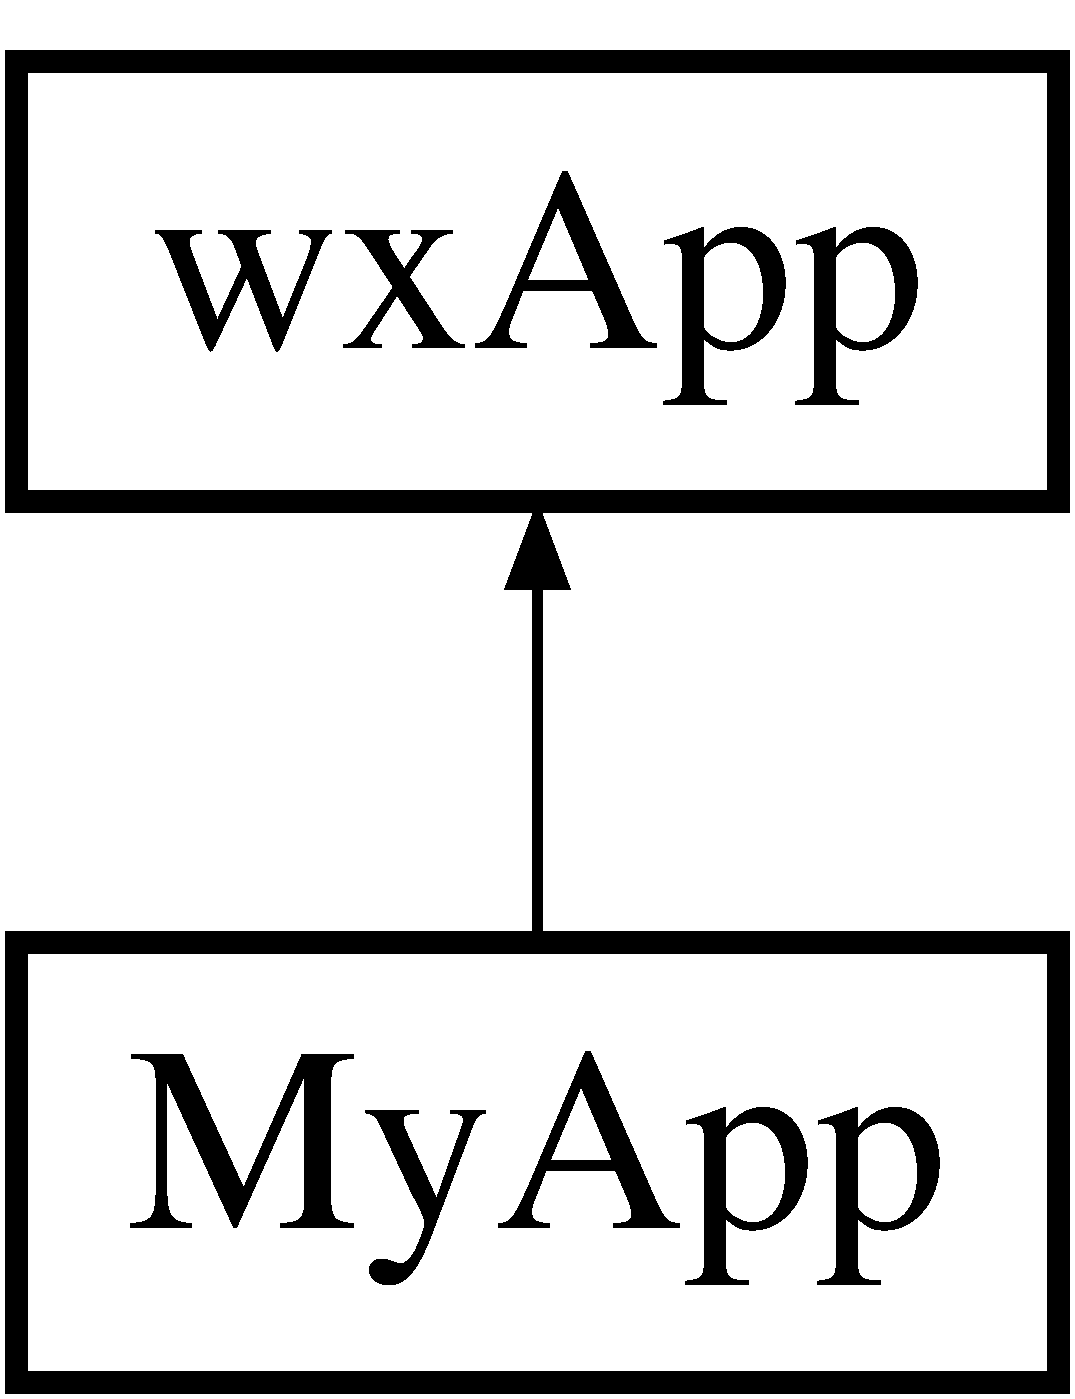
\includegraphics[height=2.000000cm]{class_my_app}
\end{center}
\end{figure}
\subsection*{Public Member Functions}
\begin{DoxyCompactItemize}
\item 
\mbox{\Hypertarget{class_my_app_a79fa75d1155f0e85e20f2869538296d6}\label{class_my_app_a79fa75d1155f0e85e20f2869538296d6}} 
virtual bool {\bfseries On\+Init} ()
\end{DoxyCompactItemize}


\subsection{Detailed Description}
main program for timer The basic class 

The documentation for this class was generated from the following file\+:\begin{DoxyCompactItemize}
\item 
main.\+cpp\end{DoxyCompactItemize}

\hypertarget{class_second_timer}{}\section{Second\+Timer Class Reference}
\label{class_second_timer}\index{Second\+Timer@{Second\+Timer}}


header for the \hyperlink{class_second_timer}{Second\+Timer} class  




{\ttfamily \#include $<$Second\+Timer.\+hpp$>$}

Inheritance diagram for Second\+Timer\+:\begin{figure}[H]
\begin{center}
\leavevmode
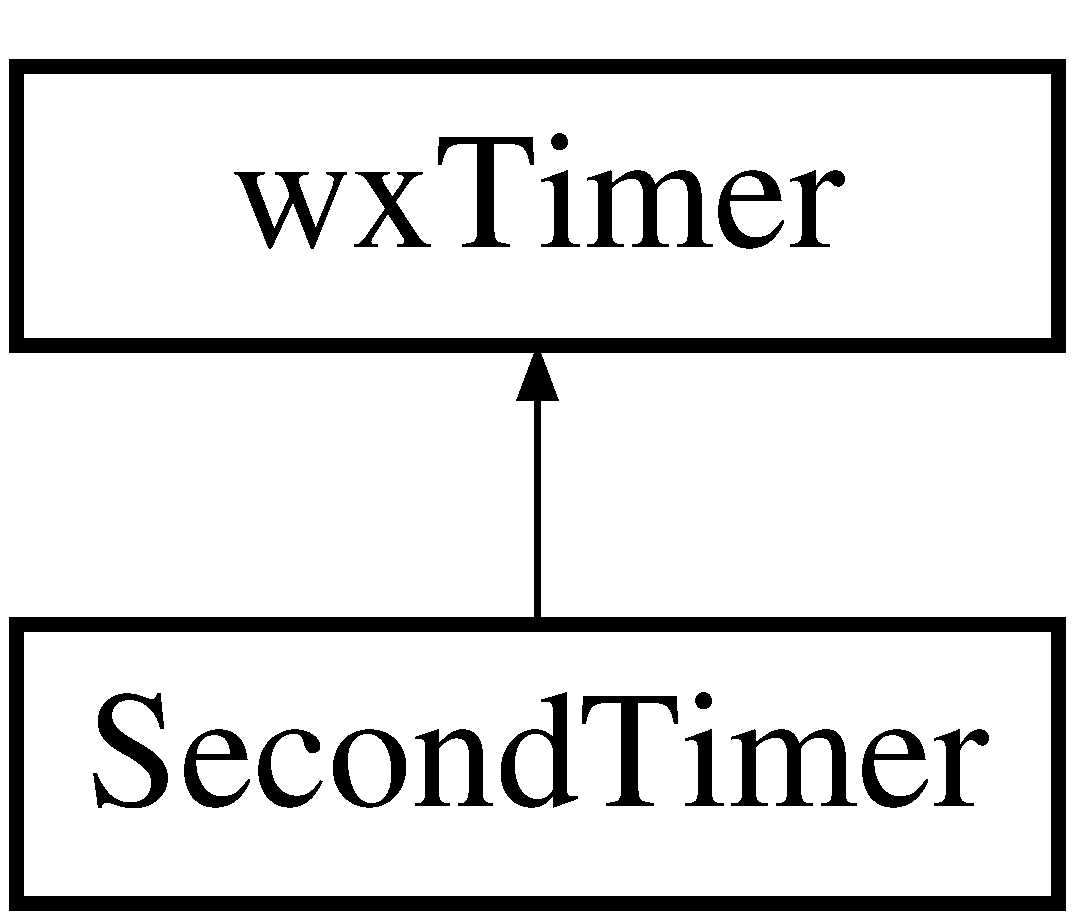
\includegraphics[height=2.000000cm]{class_second_timer}
\end{center}
\end{figure}
\subsection*{Public Member Functions}
\begin{DoxyCompactItemize}
\item 
\hyperlink{class_second_timer_ac9fadd2cf50106982c642b8142d99252}{Second\+Timer} ()
\begin{DoxyCompactList}\small\item\em Implementation of the \hyperlink{class_second_timer}{Second\+Timer} class. \end{DoxyCompactList}\item 
\hyperlink{class_second_timer_a1502fddbf09df489c7fa2e0a0e38e7cd}{$\sim$\+Second\+Timer} ()
\item 
int \hyperlink{class_second_timer_aaf1b62f5484b58c312756aa892387e63}{Start\+Timer} ()
\item 
\mbox{\Hypertarget{class_second_timer_a7d74a8e103bc219566beb0cd32aa9306}\label{class_second_timer_a7d74a8e103bc219566beb0cd32aa9306}} 
int {\bfseries Stop\+Timer} ()
\item 
int \hyperlink{class_second_timer_aa49709158917df78694a64fbbbf39c24}{Reset\+Timer} ()
\item 
\mbox{\Hypertarget{class_second_timer_a6a3221e6479e97eee4f3f4b09c3c17f8}\label{class_second_timer_a6a3221e6479e97eee4f3f4b09c3c17f8}} 
std\+::chrono\+::system\+\_\+clock\+::time\+\_\+point {\bfseries Get\+Start\+Time} ()
\item 
\mbox{\Hypertarget{class_second_timer_a905028b4987556c93d5828293afd4f1e}\label{class_second_timer_a905028b4987556c93d5828293afd4f1e}} 
std\+::chrono\+::seconds {\bfseries Seconds\+Since\+Start} ()
\end{DoxyCompactItemize}
\subsection*{Static Public Member Functions}
\begin{DoxyCompactItemize}
\item 
static std\+::string \hyperlink{class_second_timer_a9a4c3b666de65077a44c4f8048d72107}{To\+String} (const std\+::chrono\+::seconds secs)
\item 
\mbox{\Hypertarget{class_second_timer_a9ec91d25f55835a007fc5bfb1abef65f}\label{class_second_timer_a9ec91d25f55835a007fc5bfb1abef65f}} 
static std\+::string {\bfseries To\+String} (const int minutes)
\end{DoxyCompactItemize}


\subsection{Detailed Description}
header for the \hyperlink{class_second_timer}{Second\+Timer} class 

A simple class that encapsulates a wx\+Timer, and fires an event (approximately) every second. 

\subsection{Constructor \& Destructor Documentation}
\mbox{\Hypertarget{class_second_timer_ac9fadd2cf50106982c642b8142d99252}\label{class_second_timer_ac9fadd2cf50106982c642b8142d99252}} 
\index{Second\+Timer@{Second\+Timer}!Second\+Timer@{Second\+Timer}}
\index{Second\+Timer@{Second\+Timer}!Second\+Timer@{Second\+Timer}}
\subsubsection{\texorpdfstring{Second\+Timer()}{SecondTimer()}}
{\footnotesize\ttfamily Second\+Timer\+::\+Second\+Timer (\begin{DoxyParamCaption}{ }\end{DoxyParamCaption})}



Implementation of the \hyperlink{class_second_timer}{Second\+Timer} class. 

Default constructor

A simple class that encapsulates a wx\+Timer, and fires an event (approximately) every second. Default constructor \mbox{\Hypertarget{class_second_timer_a1502fddbf09df489c7fa2e0a0e38e7cd}\label{class_second_timer_a1502fddbf09df489c7fa2e0a0e38e7cd}} 
\index{Second\+Timer@{Second\+Timer}!````~Second\+Timer@{$\sim$\+Second\+Timer}}
\index{````~Second\+Timer@{$\sim$\+Second\+Timer}!Second\+Timer@{Second\+Timer}}
\subsubsection{\texorpdfstring{$\sim$\+Second\+Timer()}{~SecondTimer()}}
{\footnotesize\ttfamily Second\+Timer\+::$\sim$\+Second\+Timer (\begin{DoxyParamCaption}{ }\end{DoxyParamCaption})}

Default destructor

Desstructor 

\subsection{Member Function Documentation}
\mbox{\Hypertarget{class_second_timer_aa49709158917df78694a64fbbbf39c24}\label{class_second_timer_aa49709158917df78694a64fbbbf39c24}} 
\index{Second\+Timer@{Second\+Timer}!Reset\+Timer@{Reset\+Timer}}
\index{Reset\+Timer@{Reset\+Timer}!Second\+Timer@{Second\+Timer}}
\subsubsection{\texorpdfstring{Reset\+Timer()}{ResetTimer()}}
{\footnotesize\ttfamily int Second\+Timer\+::\+Reset\+Timer (\begin{DoxyParamCaption}{ }\end{DoxyParamCaption})}

Resets the start time of the timer \begin{DoxyReturn}{Returns}
0 
\end{DoxyReturn}
\mbox{\Hypertarget{class_second_timer_aaf1b62f5484b58c312756aa892387e63}\label{class_second_timer_aaf1b62f5484b58c312756aa892387e63}} 
\index{Second\+Timer@{Second\+Timer}!Start\+Timer@{Start\+Timer}}
\index{Start\+Timer@{Start\+Timer}!Second\+Timer@{Second\+Timer}}
\subsubsection{\texorpdfstring{Start\+Timer()}{StartTimer()}}
{\footnotesize\ttfamily int Second\+Timer\+::\+Start\+Timer (\begin{DoxyParamCaption}{ }\end{DoxyParamCaption})}

Starts the timer ticking \begin{DoxyReturn}{Returns}
0 
\end{DoxyReturn}
\mbox{\Hypertarget{class_second_timer_a9a4c3b666de65077a44c4f8048d72107}\label{class_second_timer_a9a4c3b666de65077a44c4f8048d72107}} 
\index{Second\+Timer@{Second\+Timer}!To\+String@{To\+String}}
\index{To\+String@{To\+String}!Second\+Timer@{Second\+Timer}}
\subsubsection{\texorpdfstring{To\+String()}{ToString()}}
{\footnotesize\ttfamily std\+::string Second\+Timer\+::\+To\+String (\begin{DoxyParamCaption}\item[{const std\+::chrono\+::seconds}]{secs }\end{DoxyParamCaption})\hspace{0.3cm}{\ttfamily [static]}}

converts a seconds object into a string of MM\+:SS \begin{DoxyReturn}{Returns}
a string in the format MM\+:SS 
\end{DoxyReturn}


The documentation for this class was generated from the following files\+:\begin{DoxyCompactItemize}
\item 
Second\+Timer.\+hpp\item 
Second\+Timer.\+cpp\end{DoxyCompactItemize}

\hypertarget{class_settings_frame}{}\section{Settings\+Frame Class Reference}
\label{class_settings_frame}\index{Settings\+Frame@{Settings\+Frame}}
Inheritance diagram for Settings\+Frame\+:\begin{figure}[H]
\begin{center}
\leavevmode
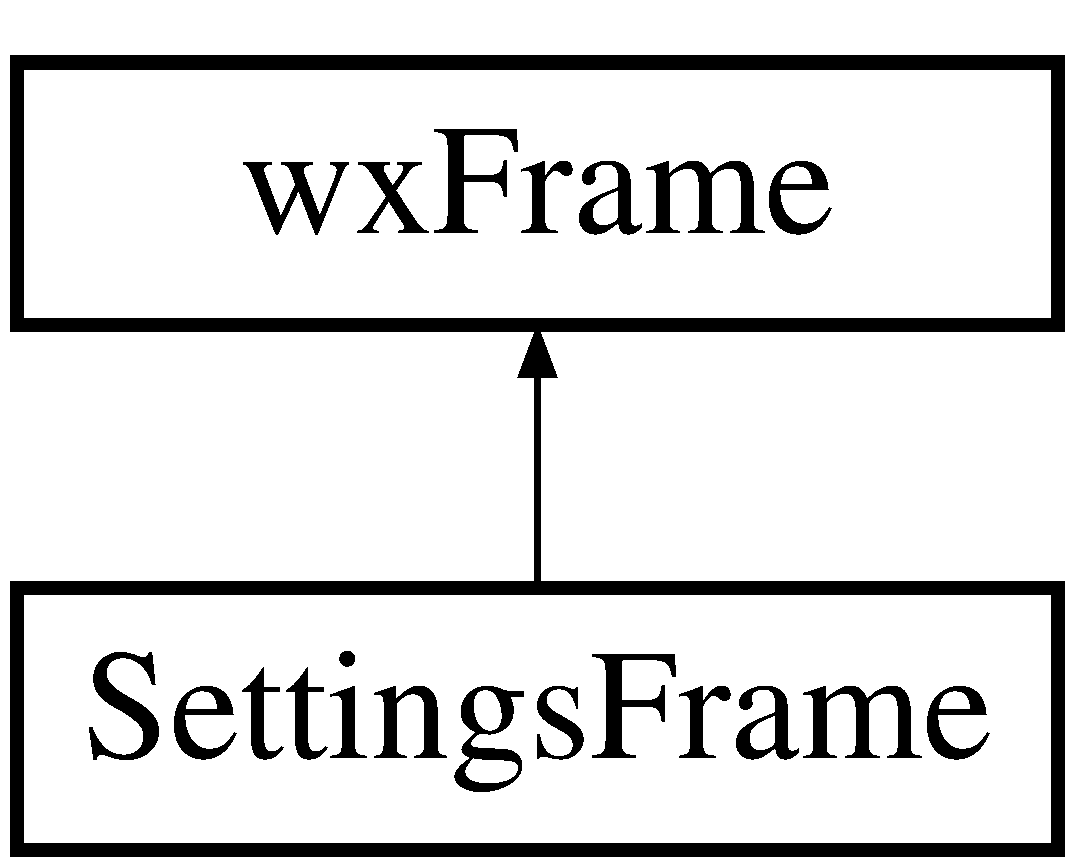
\includegraphics[height=2.000000cm]{class_settings_frame}
\end{center}
\end{figure}
\subsection*{Public Member Functions}
\begin{DoxyCompactItemize}
\item 
\mbox{\Hypertarget{class_settings_frame_a2550c773482cfd339d2bd31aca01da34}\label{class_settings_frame_a2550c773482cfd339d2bd31aca01da34}} 
{\bfseries Settings\+Frame} (const wx\+String \&window\+\_\+title)
\item 
\mbox{\Hypertarget{class_settings_frame_aa95c364d7f22e4e067d22cbce6530f68}\label{class_settings_frame_aa95c364d7f22e4e067d22cbce6530f68}} 
void {\bfseries On\+Button\+Start} (wx\+Command\+Event \&event)
\item 
\mbox{\Hypertarget{class_settings_frame_a0e22892da2b69fec0b8d35137cf18057}\label{class_settings_frame_a0e22892da2b69fec0b8d35137cf18057}} 
void {\bfseries On\+Button\+Stop} (wx\+Command\+Event \&event)
\item 
\mbox{\Hypertarget{class_settings_frame_aa3b54f55dbf67743c4ace29bd0e35a38}\label{class_settings_frame_aa3b54f55dbf67743c4ace29bd0e35a38}} 
void {\bfseries On\+Button\+Hide} (wx\+Command\+Event \&event)
\end{DoxyCompactItemize}


The documentation for this class was generated from the following files\+:\begin{DoxyCompactItemize}
\item 
Settings\+Frame.\+hpp\item 
Settings\+Frame.\+cpp\end{DoxyCompactItemize}

\hypertarget{class_text_control}{}\section{Text\+Control Class Reference}
\label{class_text_control}\index{Text\+Control@{Text\+Control}}
Inheritance diagram for Text\+Control\+:\begin{figure}[H]
\begin{center}
\leavevmode
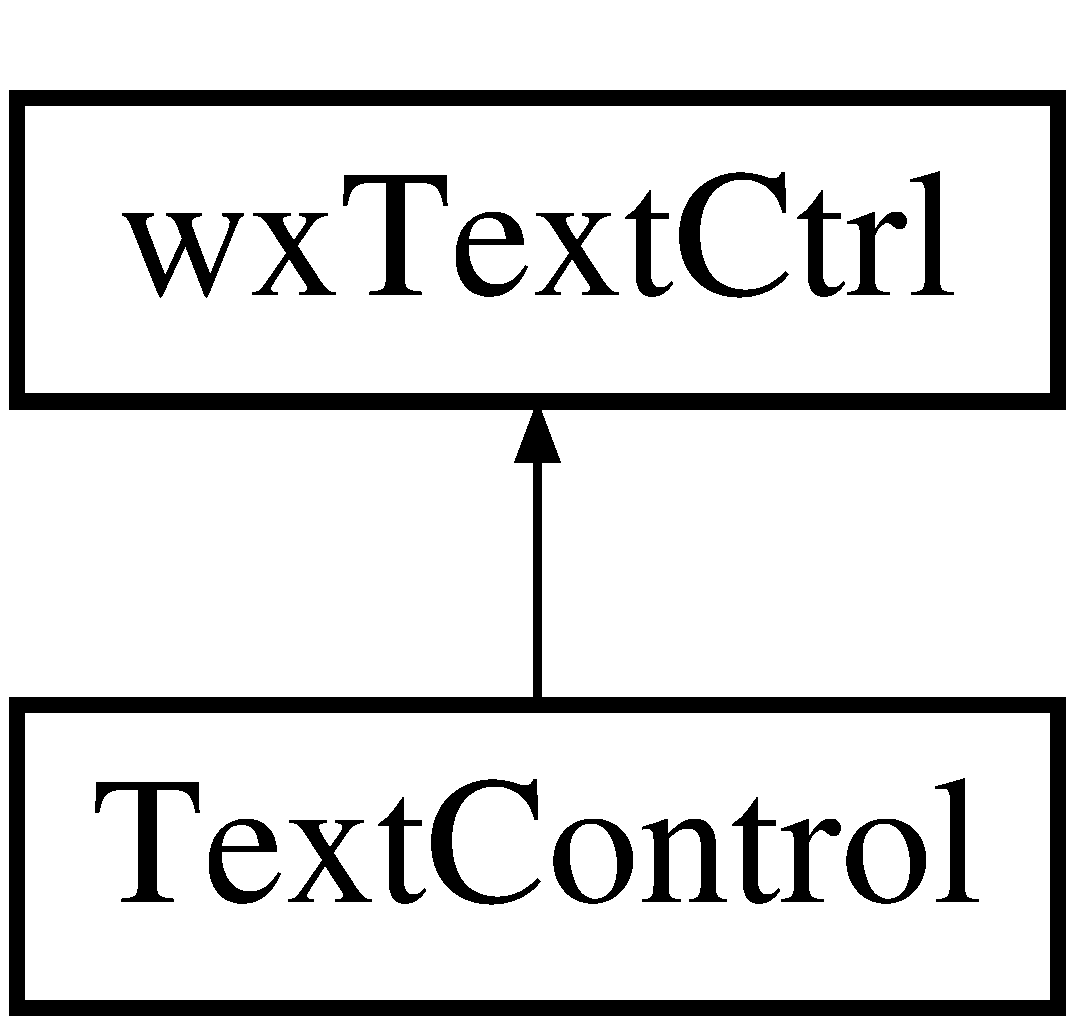
\includegraphics[height=2.000000cm]{class_text_control}
\end{center}
\end{figure}
\subsection*{Public Member Functions}
\begin{DoxyCompactItemize}
\item 
\mbox{\Hypertarget{class_text_control_ae9c393c9539be543563dab9bf19548e3}\label{class_text_control_ae9c393c9539be543563dab9bf19548e3}} 
{\bfseries Text\+Control} (wx\+Window $\ast$parent)
\item 
\mbox{\Hypertarget{class_text_control_ad8486a4d0639876fdaee57e8a7033d12}\label{class_text_control_ad8486a4d0639876fdaee57e8a7033d12}} 
{\bfseries D\+E\+C\+L\+A\+R\+E\+\_\+\+E\+V\+E\+N\+T\+\_\+\+T\+A\+B\+LE} ()
\end{DoxyCompactItemize}


The documentation for this class was generated from the following files\+:\begin{DoxyCompactItemize}
\item 
Text\+Control.\+hpp\item 
Text\+Control.\+cpp\end{DoxyCompactItemize}

\hypertarget{class_timer_frame}{}\section{Timer\+Frame Class Reference}
\label{class_timer_frame}\index{Timer\+Frame@{Timer\+Frame}}
Inheritance diagram for Timer\+Frame\+:\begin{figure}[H]
\begin{center}
\leavevmode
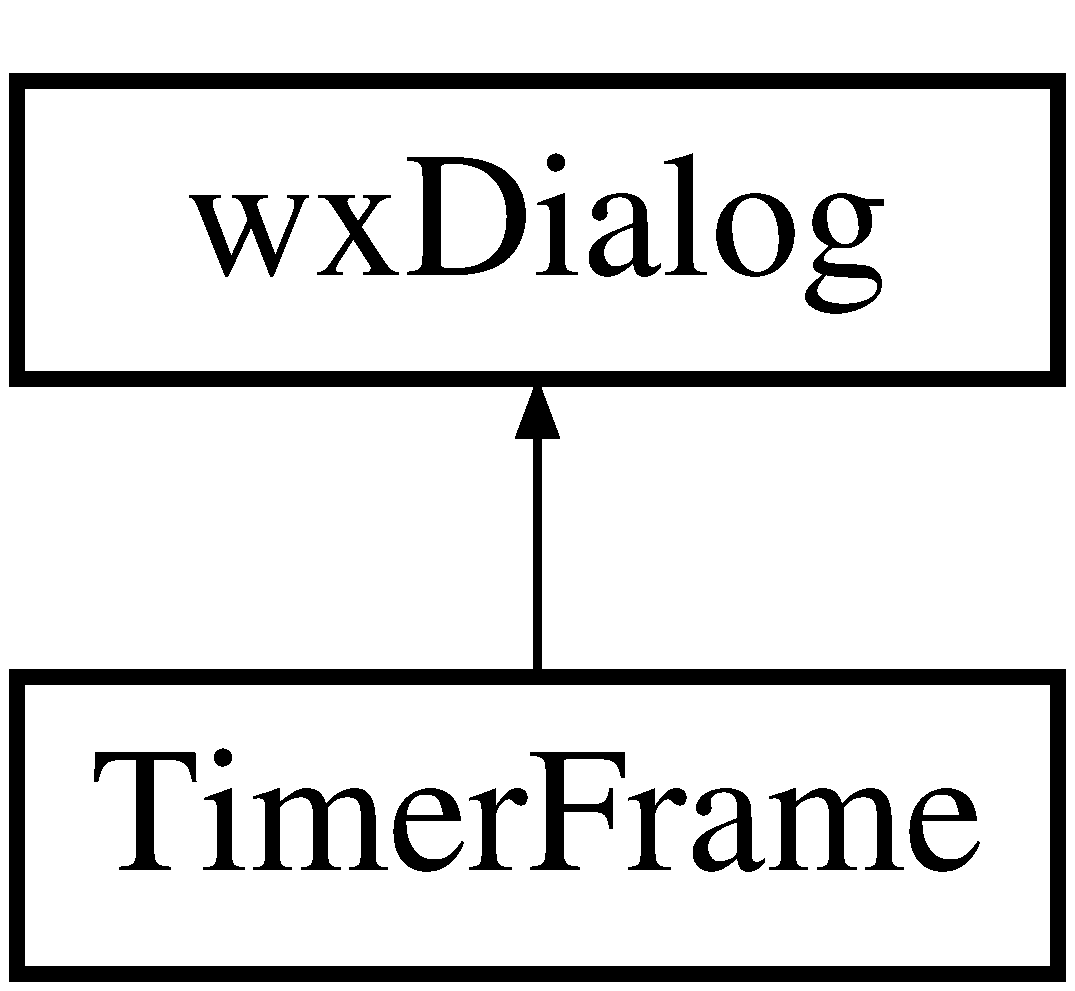
\includegraphics[height=2.000000cm]{class_timer_frame}
\end{center}
\end{figure}
\subsection*{Public Member Functions}
\begin{DoxyCompactItemize}
\item 
\mbox{\Hypertarget{class_timer_frame_a4522ee225fbef6ff57b019d41ded9170}\label{class_timer_frame_a4522ee225fbef6ff57b019d41ded9170}} 
{\bfseries Timer\+Frame} (wx\+Window $\ast$parent, \hyperlink{class_second_timer}{Second\+Timer} $\ast$second\+Timer)
\item 
\mbox{\Hypertarget{class_timer_frame_a8f10581ed95c40a528d4fab4bacab3a4}\label{class_timer_frame_a8f10581ed95c40a528d4fab4bacab3a4}} 
void {\bfseries Set\+Timer} (int minutes)
\item 
\mbox{\Hypertarget{class_timer_frame_abc95018d0407ce1cd32b2cd5e4d1c9d9}\label{class_timer_frame_abc95018d0407ce1cd32b2cd5e4d1c9d9}} 
void {\bfseries On\+Timer} (wx\+Timer\+Event \&event)
\item 
\mbox{\Hypertarget{class_timer_frame_a9060e690bf63991cf8c0a44e9fbd2adc}\label{class_timer_frame_a9060e690bf63991cf8c0a44e9fbd2adc}} 
bool {\bfseries Set\+Foreground\+Colour} (const wx\+Colour \&colour)
\end{DoxyCompactItemize}


The documentation for this class was generated from the following files\+:\begin{DoxyCompactItemize}
\item 
Timer\+Frame.\+hpp\item 
Timer\+Frame.\+cpp\end{DoxyCompactItemize}

%--- End generated contents ---

% Index
\backmatter
\newpage
\phantomsection
\clearemptydoublepage
\addcontentsline{toc}{chapter}{Index}
\printindex

\end{document}
